\documentclass[final]{anthology-ch}

\usepackage{booktabs}
\usepackage{graphicx}
\usepackage{float}
\usepackage[utf8]{inputenc}
\usepackage{pgfplots}
\pgfplotsset{compat=1.18}
\usepackage{pgfplotstable}
\usepackage{colortbl}
\usepackage{array}
\usepackage{rotating}
\usepackage{amsmath}
\usepackage{amssymb}
\usepackage{listings}
\usepackage{xcolor}
\usepackage{tcolorbox}
\usepackage{inconsolata}
\usepackage{hyperref}

\definecolor{C_Blue}{rgb}{0.22, 0.45, 0.85}
\definecolor{C_Green}{rgb}{0.0, 0.6, 0.4}
\definecolor{C_Orange}{rgb}{0.95, 0.55, 0.2}

\title{How are Literary Histories written? An LLM-based Analysis of Objects and Perspectives in German Literary History}

\author[1]{Evelyn Gius}[
orcid=0000-0001-8888-8419
]

\author[1]{Stefanie Messner}[
orcid=0009-0007-2477-7948
]

\author[2]{Axel Pichler}[
orcid=0000-0002-9177-7645
]

\affiliation{1}{Institute of Linguistics and Literary Studies, Technical University of Darmstadt, Darmstadt, Germany}
\affiliation{2}{Department of German Studies, University of Vienna, Vienna, Austria}

\keywords{literary history, classification, LLMs}

\pubyear{2025}
\pubvolume{3}
\pagestart{1074}
\pageend{1091}
\conferencename{Computational Humanities Research 2025}
\conferenceeditors{Taylor Arnold, Margherita Fantoli, and Ruben Ros}
\doi{10.63744/cUQmTV3y3P8Z}
\paperorder{63}

\addbibresource{bibliography.bib}

\begin{document}

\maketitle

\begin{abstract}
This contribution presents a case study on the LLM-based analysis of literary histories. For analyzing how literary historiography -- i.e., the writing of a literary history -- works, we examine both the objects mentioned in literary histories and the so called analytical perspective on them. With an iteratively improved pipeline based on the analysis of propositions, we use an LLM to analyze three German literary histories. We find some frequent combinations of objects and perspectives as well as a potential relation of their prominence to the overall direction of the literary history in question. Moreover, our findings show that the approach is promising for a more comprehensive analysis of literary historiography -- a central practice for Literary Studies that is debated a lot, but rarely described as a method.
\end{abstract}

\section{Introduction}
\subsection{Exploring Literary Historiography with LLMs}
This contribution presents a case study on using large language models (LLMs) for the analysis of literary histories. With this, we address two central challenges faced by the respective fields of Literary Studies and Artificial Intelligence. First, the writing of literary histories is considered one of the core practices in the field of Literary Studies, but there is also a notable lack of methodological explications on how such literary histories are actually produced. Second, LLMs appear to be a promising tool for conducting such analyses, as they have the potential to uncover the implicit structures, patterns, and analytical perspectives that shape the production of literary histories. However, considering that the domain under investigation -- recent German-language literary histories -- was most likely not part of their training data \cite{chang_speak_2023}, it is first necessary to determine how accurately such models can actually describe and analyze these texts.
Overall, literary histories are an interesting text type for probing the capacities of LLMs to support research in Literary Studies, which until now is mainly focusing on text analysis and interpretation (cf. for example \cite{walsh_sonnet_2024,jannidis_large_2025}).

Therefore, we are developing a approach where we utilize LLMs for comprehensive analyses of literary histories and test the extent to which LLMs can produce analyses of literary-historical texts that are comparable to analyses of humans. The base will be German-language literary histories on German literature. For their analysis, we formalize categories for the writing of literary histories provided by scholarly work \cite{schonert_literaturgeschichtsschreibung_2013}. Since literary histories, just like other writing in the field of Literary Studies, display a high complexity in terms of linguistic and phrase structure, which poses challenges both to human annotators and LLMs, we introduce the extraction of propositions as an intermediate step.

\subsection{Research Questions}

This case study lays the groundwork for a larger research project that explores foundational questions in the field of literary historiography with LLMs. The overarching research interest is centered around a better understanding of the methodology behind literary historiography. This includes the analysis of the writing of literary histories as an established, but little described scholarly practice. For this, scholarly work centered on the methodology will be scrutinized and an extensive analysis of descriptive, narrative, and explanatory textual practices in literary histories will be performed.

Within this broader context, in this paper we address specific research questions connected to the the usage of LLMs:
Is it possible to categorically capture both the objects of study and the analytical perspectives—a) in principle, and b) through the application of large language models (LLMs)? Furthermore, how, and to what extent, can the patterns of linking objects of study and analytical perspectives be identified in the selected examples of literary histories?

\section{Related Work}

\subsection{Methodology of Literary Historiography}
Although literary theory has identified the need for a systematic description of methodological practices for constructing a literary history as a desideratum \cite{schonert_literaturgeschichtsschreibung_2013}, it has yet to be adequately addressed. Instead, it has been described as being in crisis since the 1960s \cite{jaus_literaturgeschichte_1970, wellek_fall_1979, gumbrecht_diesseits_2004,borkowski_ziele_2013}.

In response to the absence of a generally accepted, scientifically grounded \enquote*{theory of literary historiography}, Schönert has proposed an initial conceptual framework aimed at capturing the methods employed in literary-historical writing and addressing the necessary, interest-driven reduction of complexity in historiographic representations. He argues that a theory of literary historiography must address the delineation of the object area, establish criteria for the selection of texts and events, offer models for temporal structuring, and propose approaches for contextualization and for linking literary developments to extra-literary phenomena. Building on \cite{danneberg_vom_1992,voskamp_literaturgeschichte_2000}, Schönert considers this latter aspect central; that is, the methodological question of how literary texts can be related to historical, social, and institutional conditions.

\subsection{LLM-based Classification in Computational Literary Studies}
A recent paradigm in NLP is prompt-based learning, where tasks are reformulated as prompts to leverage the capabilities of pre-trained language models. This approach has been termed \enquote*{pre-train, prompt, and predict} by Liu et al. \cite{liu2021pretrainpromptpredictsystematic}, where the input is transformed into a textual prompt with unfilled slots, and the language model generates predictions by probabilistically completing the prompt.

Classification, i.e., the assignment of a categorical label to a text passage or an entire text, is one of the central practices of Computational Literary Studies. LLMs and the \enquote*{pre-train, prompt, and predict}-approach are increasingly being used for this purpose as well. An overview of the various applications of classification using LLMs in Computational Literary Studies and Cultural Analytics is provided by \cite{bamman_classification_2024}.

\section{Formalizing Literary Historiography}
\subsection{Categories: Objects and Perspectives in Literary Histories}
For developing our framework for analyzing literary histories, we build on the initial framework proposed by Schönert \cite{schonert_literaturgeschichtsschreibung_2013}. Schönert suggests that literary historiography is characterized by different methods such as social/cultural, intellectual-historical or media historical approaches.

Since we are not yet examining methods at this stage of our project, but rather the ways in which objects are described in literary histories, we refer to them as 'analytical perspectives' (see below).
Our initial attempts to apply these categories to literary histories have revealed two key findings: First, Schönert's list of methods does not cover all the analytical perspectives employed in literary histories. In addition to those he mentions, there are also biographical, text-analytical, and poetological perspectives. Second, a review of the textual material suggests that these analytical perspectives are already realized within the texts (i.e., at the proposition level), as the object of a statement is attributed certain properties through such perspectives, meaning it is described or classified from these perspectives.

Accordingly, we develop and employ a two-dimensional semantic annotation model to annotate objects and analytical perspectives German-language literary histories.

The annotation by human annotators as well as by LLMs follows a decision tree that organizes the categories in a predefined order (see the prompt~\ref{appdx:appendix-prompt_class_eng}).

\paragraph{Object Categories.}

First, we annotate object categories. These are used to classify the object a given sequence refers to. The following categories are distinguished:

\begin{enumerate}
\item \textbf{Person}
refers to one or more individual human beings.\\
\textit{(e.g., emperor, author, citizen, merchant, Goethe)}

\item \textbf{Epoch/Movement}
refers to a literary or historical era or movement.\\
\textit{(e.g., Romanticism, Modernism, Expressionism)}

\item \textbf{Geographic Entity}
refers to a place or location.\\
\textit{(e.g., Germany, Vienna, Alps)}

\item \textbf{Political Organization}
refers to political bodies or institutions.\\
\textit{(e.g., European Union, Roman Republic, Habsburg Monarchy)}

\item \textbf{Concept/Term}
refers to an abstract idea or theoretical concept.\\
\textit{(e.g., Humanism, Nation, Postmodernism)}

\item \textbf{Historical Event}
refers to a specific historical event.\\
\textit{(e.g., French Revolution, Fall of the Berlin Wall, Thirty Years’ War)}

\item \textbf{Text}
refers to a written work or its internal elements.\\
\textit{(e.g., novel, letter, character, fictional place)}

\end{enumerate}

\paragraph{Analytical Perspectives.}
Second, we annotate analytical perspectives. Analytical perspectives describe the way an object is framed or interpreted. The following categories are distinguished:

\begin{enumerate}
\item \textbf{Intellectual Historical} refers to the object being described as an expression of the historical development of ideas, worldviews, or intellectual tendencies, or as a carrier or mediator of these.

\item \textbf{Social/Cultural Historical} refers to the object being described as shaped by social, cultural, or societal conditions, or as having influence on these contexts and not being an individual author.

\item \textbf{Methodological} refers to the object being described with regard to its methodological approach.

\item \textbf{Media Historical} refers to the object being described with regard to its technical, material, or institutional form of communication.

\item \textbf{Poetological} refers to the object being described in terms of its construction, design principles, or literary techniques.

\item \textbf{Production Aesthetic} refers to the object being an author involved in the production of a text, or a text whose genesis is thematized.

\item \textbf{Textual Analytical} refers to the object being a text that is analyzed or interpreted.

\item \textbf{Biographical} refers to the object being described in relation to the biography of a person.

\end{enumerate}

\subsection{Segments: Propositions in Literary Histories}
Our first annotation experiments with human annotators focused on
sentences as annotation spans. Due to the complexity of many sentences in the literary histories, this resulted in poor agreement.

We found it difficult to identify only one object and perspective in sentences as:
\begin{quote}
Die Vorstellung, die sich mit der Bezeichnung \enquote*{Klassik} verbindet, ist von Goethe und Schiller und durch den Ort Weimar, der im Bewusstsein der Zeitgenossen und der Nachwelt stets mit dem literarischen Schaffen von Goethe (1749–1832) und Schiller (1759–1805) assoziiert wurde, geprägt.\cite{beutin_deutsche_2013}

The concept associated with the term \enquote*{Classicism} was shaped by Goethe, Schiller, and the city of Weimar, which was always associated in the minds of contemporaries and posterity with the literary works of Goethe (1749–1832) and Schiller (1759–1805).
\end{quote}

The reduction of syntactic complexity by splitting the sentences into verb phrases with all their dependencies (i.e., minimal sentence units) yielded only small improvement. Therefore we introduced a preparatory step that could be performed by an LLM: the extraction of propositions.

In the context of this study, a \textbf{proposition} is defined as a semantically discrete, syntactically normalized statement that expresses a singular claim about a literary-historical object. Each proposition contains: a clearly identifiable object (e.g., an author or a literary work), a predicate expressing an action, characteristic, or relation, and, optionally, temporal or contextual information (for an example including the prompt and the corresponding output for the sentence above, see ~\ref{appdx:appendix-prompt-prop_extract_ger} and ~\ref{appdx:appendix-prompt-prop_extract_eng})\footnote{We apply an additive predicate interpretation, meaning that coordinated arguments (e.g., “Goethe and Schiller”) are distributed over the predicate. Thus, each conjunct yields a separate, truth-evaluable proposition.}.

\section{Data}

We work with samples of 4,000 propositions from the following three literary histories:\footnote{The data and Jupyter notebooks are available at: \url{https://github.com/AxPic/LitHist}}

\begin{itemize}
\item \textit{Neue deutsche Literaturgeschichte} by Peter J. Brenner \cite{brenner_1996}, which, according to its preface, aims to provide \enquote{enlightenment about historical developments.}
\item \textit{Deutsche Literaturgeschichte} by Wolfgang Beutin and others \cite{beutin_deutsche_2013}, which, according to the publisher's announcement, \enquote{shows the authors, their works, and the literary scene in close connection with the social, cultural, and political zeitgeist.}
\item \textit{Deutsche Literaturgeschichte} by Rainer Ruffing \cite{ruffing_deutsche_2021}, which, according to the publisher's announcement, \enquote{is aimed both at students of Literary Studies and at anyone else seeking a well-founded overview of the history of German literature.}
\end{itemize}

\section{Methods}

We employ a three-step pipeline: In the first step, individual sentences are extracted from the literature histories and transferred into a table using SpaCy. In the second step, GPT-4.1 is used to extract the propositions contained in each sentence based on this table. In the third step, these propositions are classified using GPT-4.1 according to the annotation guidelines outlined above.

This pipeline is the result of a multi-stage exploratory process. Its individual steps included the creation of annotation guidelines, their iterative refinement, the manual creation of annotated test data, and the evaluation-based selection of a model-prompt combination. The individual steps were carried out as follows:

\paragraph{Proposition Extraction.} The extraction process systematically decomposes complex or coordinated sentences into independent propositional units. It was performed using GPT-4.1. This enables targeted analysis and machine-readable representation.

Key characteristics of this propositional model include:

\begin{enumerate}
\item \textbf{Decontextualization of syntactic complexity:} Coordinated or embedded structures are resolved into elementary statements.
\item \textbf{Normalization and individuation:} Statements are standardized into a uniform form (e.g., ``X does Y at time Z''), even if the source sentence presents them in aggregated or elliptical form.
\item \textbf{Semantic reusability:} Each proposition stands alone as a self-contained unit suitable for further semantic or computational analysis.
\end{enumerate}

\paragraph{Iterative Development of Annotation Guidelines.}
The annotation guidelines were iteratively refined over six rounds of annotation of one chapter from \cite{beutin_deutsche_2013} and one chapter from \cite{brenner_1996}. The annotations were performed by the authors of this paper, who are trained in Literary Studies. After four rounds, the original idea of annotating the grammatically complete sentences from the literature histories as a whole was abandoned due to low inter-annotator agreement (Fleiss' Kappa below 60\% for both categories). In subsequent rounds, extracted propositions were annotated instead.

Additionally, two categories originally intended for annotation were ultimately discarded. The first was the category of \enquote*{Author} under the objects of analysis, which was confused with other persons. Therefore, we subsume authors under the class \enquote*{Person} in the final version.  The second was the category of \enquote*{General Historical} within the analytical perspectives, as it was consistently annotated incoherently by the tested LLMs.

\paragraph{Test Data.}
The test data were created by the three authors of this paper, who annotated 154 extracted propositions from one chapter of \cite{beutin_deutsche_2013}. After an initial round of annotation, during which the Fleiss' Kappa was calculated, one of the three annotators created silver-standard annotations based on the results.

\paragraph{Evaluation-Based Selection of a Model-Prompt Combination.}
In the final step, a prompt based on the decision tree derived from the annotation guidelines was tested in combination with three different large language models (LLMs): GPT-4.1\footnote{\url{https://platform.openai.com/docs/models/gpt-4.1}}, Mistral-Large\footnote{\url{https://mistral.ai/news/mistral-large}}, Claude-Sonnet-4\footnote{\url{https://www.anthropic.com/claude/sonnet}}, and Qwen3-VL-235B\footnote{\url{https://huggingface.co/Qwen/Qwen3-VL-235B-A22B-Instruct}}. The evaluation aimed to determine the most effective model-prompt combination by assessing the quality of the generated annotations, measured by F1, Accurcay, Precision and Recall (see \autoref{tab:model_scores}).

\begin{table}
\centering
\begin{tabular}{lcccc}
\toprule
Metric & GPT-4.1 & Claude & Mistral & Qwen3-VL-235B \\
\midrule
\multicolumn{5}{l}{\textbf{Object Domain}} \\
Accuracy  & \textbf{0.8467} & 0.8067 & 0.8000 & 0.8267 \\
Precision & \textbf{0.9083} & 0.5191 & 0.4244 & 0.4088 \\
Recall    & \textbf{0.8467} & 0.4421 & 0.4949 & 0.4846 \\
F1-Score  & \textbf{0.8696} & 0.4250 & 0.4376 & 0.4069 \\
\midrule
\multicolumn{5}{l}{\textbf{Analytical Perspective}} \\
Accuracy  & 0.6800 & 0.6533 & 0.6867 & \textbf{0.7200} \\
Precision & \textbf{0.7640} & 0.4136 & 0.2686 & 0.3641 \\
Recall    & \textbf{0.6800} & 0.3845 & 0.2457 & 0.3580 \\
F1-Score  & \textbf{0.7034} & 0.3684 & 0.2334 & 0.3278 \\
\bottomrule
\end{tabular}
\caption{Evaluation metrics for GPT-4.1, Claude, Mistral, and Qwen3-VL-235B across the Object Domain and Analytical Perspective categories. The best results for each metric are highlighted in bold.}
\label{tab:model_scores}
\end{table}

Based on these results, GPT-4.1 was selected for further evaluation. Recent studies suggest that even proprietary LLMs exhibit only limited conceptual plasticity through mere string manipulation (i.e., prompt engineering). In other words, a semantic shift in the meaning of technical terms through redefinitions or explications of these terms is not always fully achievable. For this reason, we refrained from extensive prompt engineering. This evaluation was therefore conducted in three different setups: first, using a reduced prompt created by ChatGPT with the help of selected examples; second, in a two-step process where the object domain was determined first, followed by the analytical perspective; and third, by taking into account the context of each proposition, i.e., the full sentence from which the proposition was originally extracted (see \autoref{tab:second_test_run}).

\begin{table}
\centering
\begin{tabular}{lccc}
\toprule
Metric & GPT-4.1 (Reduced Prompt) & GPT-4.1 (Two-Step) & GPT-4.1 (Context) \\
\midrule
\multicolumn{4}{l}{\textbf{Object Domain}} \\
Accuracy  & 0.8600 & 0.8333 & \textbf{0.8667} \\
Precision & 0.9280 & \textbf{0.9311} & 0.9308 \\
Recall    & 0.8600 & 0.8333 & \textbf{0.8667} \\
F1-Score  & 0.8797 & 0.8702 & \textbf{0.8894} \\
\midrule
\multicolumn{4}{l}{\textbf{Analytical Perspective}} \\
Accuracy  & \textbf{0.7267} & 0.7133 & 0.6800 \\
Precision & \textbf{0.7477} & 0.7170 & 0.7318 \\
Recall    & \textbf{0.7267} & 0.7133 & 0.6800 \\
F1-Score  & \textbf{0.7256} & 0.7091 & 0.6894 \\
\bottomrule
\end{tabular}
\caption{Evaluation metrics for GPT-4.1 in the second test run across three setups: reduced prompt, two-step process, and context-based evaluation. The best results for each metric are highlighted in bold.}
\label{tab:second_test_run}
\end{table}

Since the performance gain achieved with these variations was minimal and, moreover, not consistent across both domains, we ultimately decided to retain the combination of GPT-4.1 with the prompt based on the annotation guidelines (see the prompt~\ref{appdx:appendix-prompt_class_eng}). This approach provided a balanced and reliable performance for both the Object Domain and Analytical Perspective categories, aligning well with the goals of our study.

\section{Results}

The data analysis of 4,000 propositions from \cite{brenner_1996},\cite{beutin_deutsche_2013}and \cite{ruffing_deutsche_2021} reveals the following patterns across the examined samples.

\paragraph{Distribution of objects and analytical perspectives.}
In all three samples, the four most frequent representatives of the category \emph{objects of analysis} are not only identical but -- except for two minor variations -- ranked in the same order (cf. \autoref{tab:category_percentage_comparison} and \autoref{fig:top3_category_percentage_comparison}). In the Beutin and Ruffing samples, the most dominant object is \emph{text}, followed by \emph{concept/term} and \emph{person}. In the Brenner sample, the first two positions are reversed, though the difference in percentage is only 0.12\%. Notably, \emph{text} accounts for the largest share in two of the three samples, while \emph{person} represents approximately one-fourth of the objects in all samples. Contrary to the frequently proclaimed theoretical \enquote*{turns,} text continues to play a central role in these literary histories. The same holds true for the category of \emph{person}, which literary historiography evidently still relies on -- despite the oft-cited \enquote*{death of the author.}\footnote{German-language scholarship has already shown that, despite theoretical critiques of the author concept, the author continues to play a significant role in interpretive practice (cf. \cite{willand_autorfunktionen_2011}).}

The situation is somewhat different with regard to \emph{analytical perspectives} (cf. \autoref{tab:percentage_analytical_perspectives} and \autoref{fig:top5_analytical_perspectives_percentage}). Although the same five categories appear most frequently across all samples, their rankings differ. In the Ruffing and Brenner samples, the dominant perspective is intellectual historical; in contrast, the Beutin sample is led by a social/cultural historical perspective. This aligns with Beutin’s own description of his historiographical approach. However, the dominance of this perspective at the level of propositions is notably less pronounced than expected: while roughly 25\% of Beutin’s propositions reflect a social/cultural perspective, around 22\% adopt an intellectual historical-based one.

\begin{table}
\centering
\begin{tabular}{lccc}
\toprule
\textbf{Object} & \textbf{Brenner (\%)} & \textbf{Beutin (\%)} & \textbf{Ruffing (\%)} \\
\midrule
\textbf{Text}                        & 32.03\% & \textbf{31.15\%} & \textbf{30.43}\% \\
Concept/Term                      & \textbf{32.15}\%          & 30.68\%          & 23.28\% \\
Person                               & 24.55\%          & 24.78\%          & 29.78\% \\
Epoch/Movement                      & 4.68\%           & 4.83\%           & 10.10\% \\
Historical Event                             & 3.15\%           & 4.33\%           & 2.70\% \\
Geographic Entity                & 2.45\%           & 2.63\%           & 2.83\% \\
Political Organization      & 0.50\%           & 1.15\%           & 0.25\% \\
Not Classifiable                   & 0.45\%           & 0.45\%           & 0.63\% \\
Hallucinated labels                  & 0.05\%          & 0.03\%                 & 0.03\% \\
\bottomrule
\end{tabular}
\caption{Percentage distribution of categories across the texts by Brenner, Beutin, and Ruffing. The most frequent category for each text is highlighted in bold.}
\label{tab:category_percentage_comparison}
\end{table}




\begin{figure}[H]
    \centering
    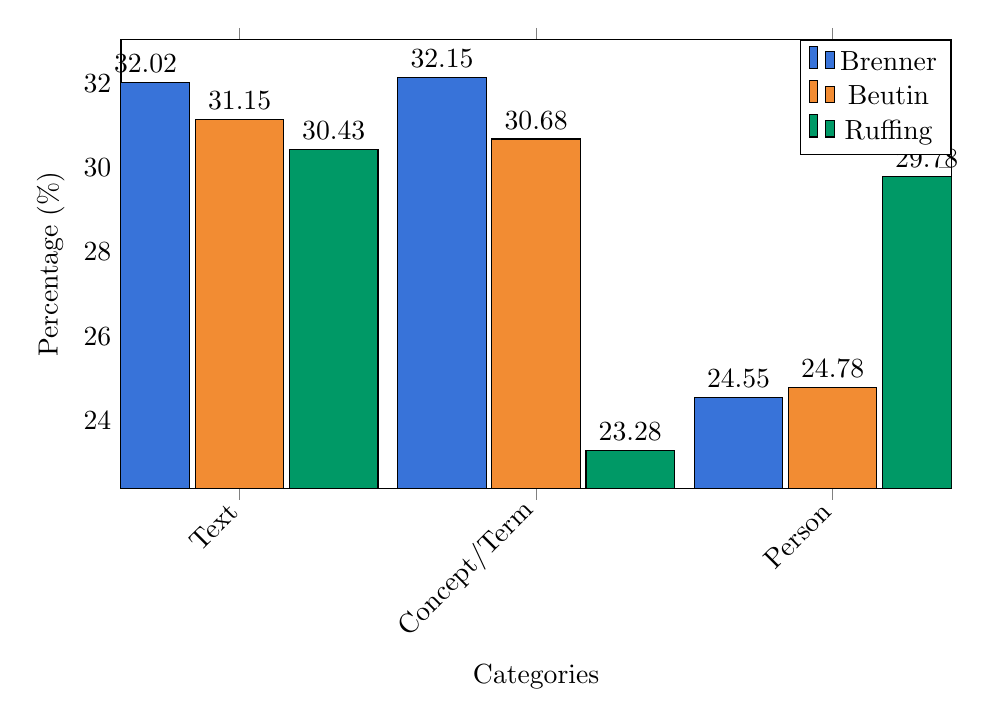
\begin{tikzpicture}
        \begin{axis}[
            ybar,
            bar width=32pt, % Balkenbreite verdoppelt
            width=\textwidth,
            height=0.6\textwidth,
            enlarge x limits=0.2,
            legend style={at={(1,1)}, anchor=north east},
            ylabel={Percentage (\%)},
            xlabel={Categories},
            symbolic x coords={Text, Concept/Term, Person},
            xtick=data,
            x tick label style={rotate=45, anchor=east},
            nodes near coords,
            nodes near coords align={vertical},
        ]
            % Daten für Brenner
            \addplot[fill=C_Blue] coordinates {
                (Text, 32.02) (Concept/Term, 32.15) (Person, 24.55)
            };
            % Daten für Beutin
            \addplot[fill=C_Orange] coordinates {
                (Text, 31.15) (Concept/Term, 30.68) (Person, 24.78)
            };
            % Daten für Ruffing
            \addplot[fill=C_Green] coordinates {
                (Text, 30.43) (Concept/Term, 23.28) (Person, 29.78)
            };

            % Legende
            \legend{Brenner, Beutin, Ruffing}
        \end{axis}
    \end{tikzpicture}
    \caption{Percentage distribution of the Top-3 objects (Text, Concept/Term, Person) across the texts by Brenner, Beutin, and Ruffing.}
    \label{fig:top3_category_percentage_comparison}
\end{figure}

\begin{table}[H]
    \centering
    \begin{tabular}{lccc}
        \toprule
        \textbf{Analytical Perspective} & \textbf{Brenner (\%)} & \textbf{Beutin (\%)} & \textbf{Ruffing (\%)} \\
        \midrule
        Intellectual Historical      & \textbf{33,85\%}      & 21.80\%              & \textbf{34.03\%}      \\
        Poetological                     & 21.45\%               & 17.68\%              & 12.45\%               \\
        Social/Cultural Historical      & 13.55\%               & \textbf{24.23\%}     & 11.38\%               \\
        Biographical                     & 10.80\%               & 8.93\%               & 14.35\%               \\
        Textual Analytical                   & 7.55\%                & 12.85\%              & 18.10\%               \\
        Production Aesthetic            & 6.20\%                & 5.98\%               & 3.00\%                \\
        Media Historical              & 5,025\%                & 6.45\%               & 1.23\%                \\
        Not Classifiable               & 1.25\%                & 1.73\%               & 4.70\%                \\
        Methodological                   & 0.05\%                & 0.35\%               & 0.08\%                \\
        Hallucinated labels                 & 0.28\%                 & -               & 0.30\%                     \\
        \bottomrule
    \end{tabular}
    \caption{Percentage distribution of analytical perspectives across the texts by Brenner, Beutin, and Ruffing. The most frequent category for each text is highlighted in bold.}
    \label{tab:percentage_analytical_perspectives}
\end{table}

\begin{figure}[H]
    \centering
    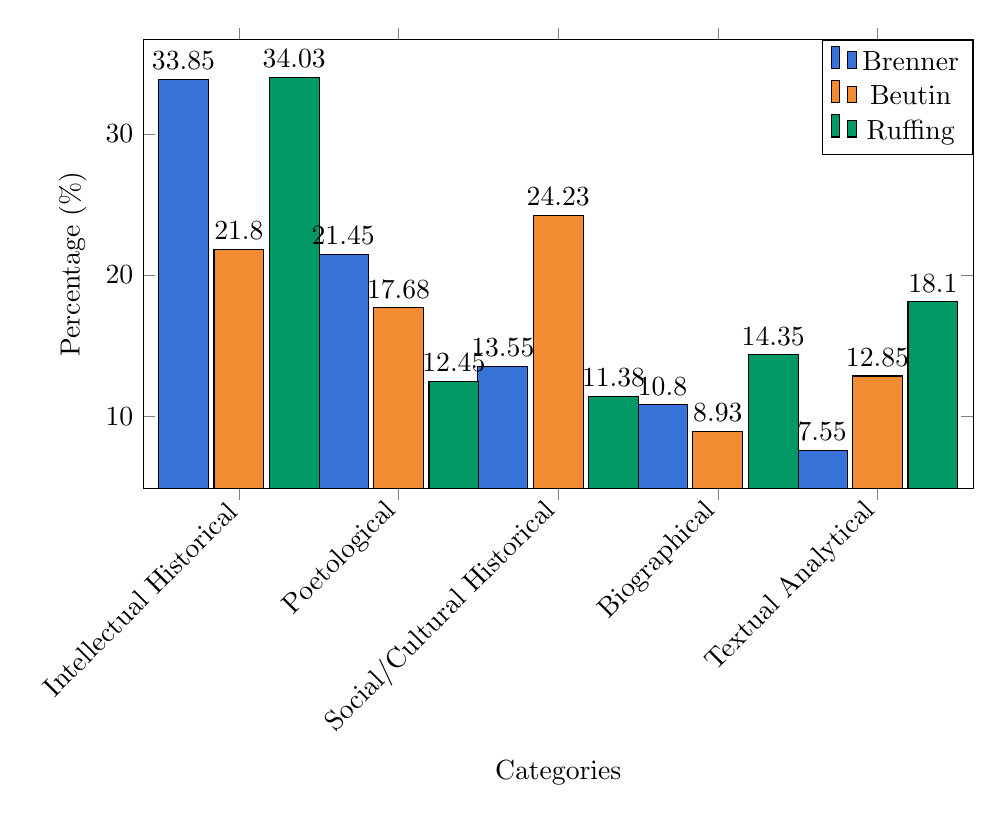
\begin{tikzpicture}
      \begin{axis}[
        ybar,
        bar width=18pt,
        width=\textwidth,
        height=0.6\textwidth,
        enlarge x limits=0.15,
        legend style={at={(1,1)}, anchor=north east}, % <-- comma added
        ylabel={Percentage (\%)},
        xlabel={Categories},
        symbolic x coords={Intellectual Historical, Poetological, Social/Cultural Historical, Biographical, Textual Analytical},
        xtick=data,
        x tick label style={rotate=45, anchor=east},
        nodes near coords,
        nodes near coords align={vertical},
      ]
            % Daten für Brenner
            \addplot[fill=C_Blue] coordinates {
                (Intellectual Historical, 33.85) 
                (Poetological, 21.45) 
                (Social/Cultural Historical, 13.55)
                (Biographical, 10.80) 
                (Textual Analytical, 7.55)
            };
            % Daten für Beutin
            \addplot[fill=C_Orange] coordinates {
                (Intellectual Historical, 21.80) 
                (Poetological, 17.68) 
                (Social/Cultural Historical, 24.23) 
                (Biographical, 8.93) 
                (Textual Analytical, 12.85)
            };
            % Daten für Ruffing
            \addplot[fill=C_Green] coordinates {
                (Intellectual Historical, 34.03) 
                (Poetological, 12.45) 
                (Social/Cultural Historical, 11.38) 
                (Biographical, 14.35) 
                (Textual Analytical, 18.10)
            };

            % Legende
            \legend{Brenner, Beutin, Ruffing}
        \end{axis}
    \end{tikzpicture}
    \caption{Percentage distribution of the Top-5 analytical perspectives (Intellectual Historical, Poetological, Social/Cultural Historical, Biographical, Textual Analytical) across the texts by Brenner, Beutin, and Ruffing.}
    \label{fig:top5_analytical_perspectives_percentage}
\end{figure}


\paragraph{Distribution of combinations of objects and analytical perspectives.}
The combinations of object and analytical perspective reveal some interesting patterns.

\begin{enumerate}
\item  In all three samples, the same analytical perspective dominates with regard to three objects: concepts/terms are predominantly treated from an intellectual history perspective. However, the intensity of this focus varies significantly, with almost 73\% in Ruffing \cite{ruffing_deutsche_2021}, 58\% in Brenner \cite{brenner_1996}, and only 39\% in Beutin \cite{beutin_deutsche_2013}. In the latter, consistent with its self-description, 36\% of the discussions of concepts/terms also take place from a social/cultural-historical perspective.

The combination of person and biographical perspective is closer in percentage terms. In all three samples, discussions of this object category occur between 35\% and 45\% from a biographical perspective. A similar pattern is observed for the combination of epoch/movement and intellectual history. In the three samples, this combination ranges between 57\% and 68\%.

\item Variations of interest can be observed with regard to the object domains of text and event. While Brenner \cite{brenner_1996} and Beutin \cite{beutin_deutsche_2013} predominantly adopt a poetological perspective on texts -- at 49\% and 39\%, respectively -- Ruffing \cite{ruffing_deutsche_2021} approaches them more from a textual-analytical perspective. This may be due to the fact that Ruffing's work is a literary history primarily aimed at undergraduate students, whereas the other two texts target a broader academic audience.

A different distribution emerges with regard to events: Brenner describes them from an intellectual history perspective, a fact that further emphasizes the dominance of this approach in his work. In contrast, Beutin and Ruffing describe events from a social/cultural historical perspective.
\end{enumerate}

\begin{table}[ht]
\centering
\caption{Reduced heat map (Brenner \cite{brenner_1996}): Highest percentage value per row highlighted}
\label{tab:reduced_heatmap}
\scriptsize
\resizebox{\textwidth}{!}{
\begin{tabular}{l>{\centering\arraybackslash}m{1.5cm}>{\centering\arraybackslash}m{1.5cm}>{\centering\arraybackslash}m{1.5cm}>{\centering\arraybackslash}m{1.5cm}>{\centering\arraybackslash}m{1.5cm}}
\toprule
\textbf{Gegenstand} &
\rotatebox{90}{Intellectual Historical} &
\rotatebox{90}{Poetological} &
\rotatebox{90}{Social/Cultural Historical} &
\rotatebox{90}{Biographical} &
\rotatebox{90}{Textual Analytical} \\
\midrule
Text & 12.3 & \cellcolor{blue!25}49.0 & 5.0 & 1.2 & 20.5 \\
Concept/Term & \cellcolor{blue!25}58.5 & 10.3 & 21.5 & 0.0 & 0.6 \\
Person & 24.6 & 5.4 & 6.4 & \cellcolor{blue!25}42.1 & 2.7 \\
Epoch/Movement & \cellcolor{blue!25}67.4 & 17.6 & 8.0 & 2.1 & 0.0 \\
Historical Event & \cellcolor{blue!25}48.4 & 0.0 & 38.1 & 0.0 & 3.2 \\
\bottomrule
\end{tabular}
}
\end{table}

\begin{table}[ht]
\centering
\caption{Reduced heat map (Beutin \cite{beutin_deutsche_2013}): Highest percentage value per row highlighted}
\label{tab:reduced_heatmap}
\scriptsize
\resizebox{\textwidth}{!}{
\begin{tabular}{l>{\centering\arraybackslash}m{1.5cm}>{\centering\arraybackslash}m{1.5cm}>{\centering\arraybackslash}m{1.5cm}>{\centering\arraybackslash}m{1.5cm}>{\centering\arraybackslash}m{1.5cm}}
\toprule
\textbf{Gegenstand} &
\rotatebox{90}{Intellectual Historical} &
\rotatebox{90}{Poetological} &
\rotatebox{90}{Social/Cultural Historical} &
\rotatebox{90}{Biographical} &
\rotatebox{90}{Textual Analytical} \\
\midrule
Text & 3.7 & \cellcolor{blue!25}39.4 & 4.6 & 0.3 & 34.7 \\
Concept/Term & \cellcolor{blue!25}39.4 & 13.2 & 35.6 & 0.0 & 0.6 \\
Person & 17.0 & 3.1 & 19.7 & \cellcolor{blue!25}35.6 & 7.3 \\
Epoch/Movement & \cellcolor{blue!25}60.6 & 11.9 & 23.8 & 0.0 & 0.0 \\
Historical Event & 20.8 & 0.0 & \cellcolor{blue!25}63.0 & 0.0 & 1.7 \\
\bottomrule
\end{tabular}
}
\end{table}

\begin{table}[ht]
\centering
\caption{Reduced heat map (Ruffing \cite{ruffing_deutsche_2021}): Highest percentage value per row highlighted}
\label{tab:reduced_heatmap}
\scriptsize
\resizebox{\textwidth}{!}{
\begin{tabular}{l>{\centering\arraybackslash}m{1.5cm}>{\centering\arraybackslash}m{1.5cm}>{\centering\arraybackslash}m{1.5cm}>{\centering\arraybackslash}m{1.5cm}>{\centering\arraybackslash}m{1.5cm}}
\toprule
\textbf{Gegenstand} &
\rotatebox{90}{Intellectual Historical} &
\rotatebox{90}{Poetological} &
\rotatebox{90}{Social/Cultural Historical} &
\rotatebox{90}{Biographical} &
\rotatebox{90}{Textual Analytical} \\
\midrule
Text & 7.7 & 21.0 & 3.5 & 2.0 & \cellcolor{blue!25}56.1 \\
Concept/Term & \cellcolor{blue!25}72.8 & 7.5 & 15.4 & 0.2 & 0.3 \\
Person & 27.0 & 7.1 & 6.6 & \cellcolor{blue!25}44.8 & 2.7 \\
Epoch/Movement & \cellcolor{blue!25}57.4 & 21.0 & 15.1 & 1.2 & 0.0 \\
Historical Event & 30.6 & 2.8 & \cellcolor{blue!25}50.9 & 2.8 & 5.6 \\
\bottomrule
\end{tabular}
}
\end{table}

\section{Outlook}
The analysis of objects and analytical perspectives in literary histories using large language models (LLMs) has proven effective, although significant development was required for the pipeline, particularly for perspective detection. The introduction of propositions led to substantial improvements in the system’s performance. Future work will focus both on grounding and broadening the approach. Methodologically, this involves experimenting with prompt optimization techniques and fine-tuning, as well as adapting smaller open-source LLMs such as OLMo. \cite{groeneveld2024olmoacceleratingsciencelanguage}. From a Literary Studies perspective, the inclusion and comparison of a wider range of texts, including counter-canonical literary histories, is an obvious next step. Moreover, future research will address the strategies for linking texts and objects within literary histories. This focus on narrative strategies has the potential to open up entirely new perspectives on literary history and enhance the interpretability and impact of our models.

\section{Limitations}

This contribution presents a work-in-progress research project and, as such, comes with several limitations. First, the inter-annotator agreement (IAA) is still not optimal -- an outcome that reflects the inherent complexity of the task but also indicates clear potential for refinement. Second, the analysis is based on only three samples, which limits the generalizability of the findings. Third, the extracted propositions have not yet undergone manual evaluation. Finally, the use of a proprietary large language model (LLM) raises legitimate concerns regarding transparency reproducibility.

\section{Author Contribution}

\begin{description}
\item[\textbf{Evelyn Gius:}] conceptualization, methodology, writing – original, review and editing
\item[\textbf{Stefanie Messner:}] conceptualization, methodology, data curation, writing – original, review and editing
\item[\textbf{Axel Pichler:}] conceptualization, methodology, formal analysis, data curation, writing – original, review and editing
\end{description}

\printbibliography

\appendix

\section{Prompt Templates}\label{appdx:appendix-prompts}

\lstset{
basicstyle=\ttfamily\small,
breaklines=true,
frame=single,
backgroundcolor=\color{gray!10},
keywordstyle=\color{blue},
commentstyle=\color{green!50!black},
stringstyle=\color{red},
showstringspaces=false
}

\tcbset{
colback=gray!10,
colframe=black,
fonttitle=\bfseries,
coltitle=black,
boxrule=0.5mm,
arc=2mm,
left=2mm,
right=2mm,
top=2mm,
bottom=2mm
}

\subsection{Prompt for Proposition Extraction (German)}\label{appdx:appendix-prompt-prop_extract_ger}
\texttt{Extrahiere aus dem folgenden Satz die Propositionen.}

\begin{itemize}
\item \texttt{Gib ausschließlich vollständige, konkrete Aussagen wieder.}
\item \texttt{Zerlege den Satz so, dass jede Aussage eine eigene, nummerierte Proposition ergibt.}
\item \texttt{Ignoriere Satzfragmente, Überschriften oder rein nominale Konstruktionen ohne Prädikat.}
\item \texttt{Trenne auch Teilaussagen, wenn sie sich auf unterschiedliche Entitäten beziehen.}
\item \texttt{Gib ausschließlich die nummerierten Propositionen aus – keine Kommentare, keine Einleitungen, keine Metabemerkungen.}
\end{itemize}

\texttt{\textbf{Satz:}} \texttt{\{satz\}}

\texttt{\textbf{Output:}}

\begin{enumerate}
\item \texttt{Die Vorstellung, die sich mit der Bezeichnung ›Klassik‹ verbindet, ist von Goethe geprägt.}
\item \texttt{Die Vorstellung, die sich mit der Bezeichnung ›Klassik‹ verbindet, ist von Schiller geprägt.}
\item \texttt{Die Vorstellung, die sich mit der Bezeichnung ›Klassik‹ verbindet, ist durch den Ort Weimar geprägt.}
\item \texttt{Der Ort Weimar wurde im Bewusstsein der Zeitgenossen stets mit dem literarischen Schaffen von Goethe assoziiert.}
\item \texttt{Der Ort Weimar wurde im Bewusstsein der Zeitgenossen stets mit dem literarischen Schaffen von Schiller assoziiert.}
\item \texttt{Der Ort Weimar wurde im Bewusstsein der Nachwelt stets mit dem literarischen Schaffen von Goethe assoziiert.}
\item \texttt{Der Ort Weimar wurde im Bewusstsein der Nachwelt stets mit dem literarischen Schaffen von Schiller assoziiert.}
\end{enumerate}

\subsection{Prompt for Proposition Extraction (English)}\label{appdx:appendix-prompt-prop_extract_eng}
\texttt{Extract the propositions from the following sentence.}

\begin{itemize}
\item \texttt{Provide only complete, concrete statements.}
\item \texttt{Break down the sentence so that each statement becomes its own numbered proposition.}
\item \texttt{Ignore sentence fragments, headings, or purely nominal constructions without a predicate.}
\item \texttt{Also separate sub-statements if they refer to different entities.}
\item \texttt{Output only the numbered propositions – no comments, no introductions, no meta-remarks.}
\end{itemize}

\texttt{\textbf{Sentence:}} \texttt{\{sentence\}}

\texttt{\textbf{Output:}}

\begin{enumerate}
\item \texttt{The concept associated with the term "Classicism" was shaped by Goethe.}
\item \texttt{The concept associated with the term "Classicism" was shaped by Schiller.}
\item \texttt{The concept associated with the term "Classicism" was shaped by the city of Weimar.}
\item \texttt{The city of Weimar was always associated in the minds of contemporaries with the literary works of Goethe.}
\item \texttt{The city of Weimar was always associated in the minds of contemporaries with the literary works of Schiller.}
\item \texttt{The city of Weimar was always associated in the minds of posterity with the literary works of Goethe.}
\item \texttt{The city of Weimar was always associated in the minds of posterity with the literary works of Schiller.}
\end{enumerate}

\subsection{Prompt for Classification (German)}\label{appdx:appendix-prompt_class_ger}
\texttt{Deine Aufgabe besteht darin, einzelne Sätze aus Literaturgeschichten im Hinblick auf ihren Gegenstand und ihre analytische Perspektive zu klassifizieren.}

\texttt{Analysiere den folgenden Satz und klassifiziere ihn entlang des folgenden Entscheidungswegs. Gib zwei Klassifikationen aus:}

\begin{itemize}
\item \texttt{\textbf{1. Gegenstand} (Worauf bezieht sich die Aussage?)}
\item \texttt{\textbf{2. Analytische Perspektive} (Wie wird dieser Gegenstand beschrieben?)}
\end{itemize}

\texttt{\textbf{Gegenstand}}

\begin{itemize}
\item \texttt{\textbf{Frage 1:} Bezieht sie sich auf einen identifizierbaren Gegenstand?}
\begin{itemize}
\item \texttt{→ Ja → weiter mit Frage 2}
\item \texttt{→ Nein → <nicht entscheidbar> bzw. <nicht anwendbar>}
\end{itemize}
\item \texttt{\textbf{Frage 2:} Bezieht sich der Satz auf eine Epoche oder literarische Strömung (z.B. Romantik, Moderne, Expressionismus)?}
\begin{itemize}
\item \texttt{→ Ja → <Epoche/Strömung>}
\item \texttt{→ Nein → weiter mit Frage 3}
\end{itemize}
\item \texttt{\textbf{Frage 3:} Bezieht sich der Satz auf eine geographische Entität (Länder, Städte, Orte)?}
\begin{itemize}
\item \texttt{→ Ja → <Geographische Entität>}
\item \texttt{→ Nein → weiter mit Frage 4}
\end{itemize}
\item \texttt{\textbf{Frage 4:} Bezieht sich der Satz auf eine politische Organisation oder einen Verband (z.B. EU, römische Republik, Habsburger)?}
\begin{itemize}
\item \texttt{→ Ja → <Politische Organisationseinheit>}
\item \texttt{→ Nein → weiter mit Frage 5}
\end{itemize}
\item \texttt{\textbf{Frage 5:} Bezieht sich der Satz auf einen Begriff oder ein abstraktes Konzept (z.B. Humanismus, Nation, Postmoderne)?}
\begin{itemize}
\item \texttt{→ Ja → <Begriff/Konzept>}
\item \texttt{→ Nein → weiter mit Frage 6}
\end{itemize}
\item \texttt{\textbf{Frage 6:} Bezieht sich der Satz auf ein historisches Ereignis (z.B. Französische Revolution, Mauerfall, 30-jähriger Krieg)?}
\begin{itemize}
\item \texttt{→ Ja → <Ereignis>}
\item \texttt{→ Nein → weiter mit Frage 7}
\end{itemize}
\item \texttt{\textbf{Frage 7:} Bezieht sich der Satz auf einen Text (z.B. Roman, Brief) oder Entitäten aus einem Text (z.B. Figuren, Orte)?}
\begin{itemize}
\item \texttt{→ Ja → <Text>}
\item \texttt{→ Nein → weiter mit Frage 8}
\end{itemize}
\item \texttt{\textbf{Frage 8:} Bezieht sich der Satz auf ein menschliches Individuum (z.B. Kaiser, Bürgerin, Kaufmann oder deren Eigenname)?}
\begin{itemize}
\item \texttt{→ Ja → <Person>}
\item \texttt{→ Nein → <nicht entscheidbar>}
\end{itemize}
\end{itemize}

\texttt{\textbf{Analytische Perspektive}}

\begin{itemize}
\item \texttt{\textbf{Frage 9:} Wird der Gegenstand als Ausdruck der historischen Entwicklung von Ideen, Weltanschauungen und geistigen Tendenzen beschrieben oder ist er Träger/Vermittler derselben?}
\begin{itemize}
\item \texttt{→ Ja → <geistes-/ideengeschichtlich>}
\item \texttt{→ Nein → weiter mit Frage 10}
\end{itemize}
\item \texttt{\textbf{Frage 10:} Wird der Gegenstand als durch gesellschaftliche, soziale oder kulturelle Bedingungen geprägt dargestellt oder wird dem Gegenstand selbst Einfluss auf diese Kontexte zugeschrieben und ist kein einzelner Autor?}
\begin{itemize}
\item \texttt{→ Ja → <sozial-/kulturgeschichtlich>}
\item \texttt{→ Nein → weiter mit Frage 11}
\end{itemize}
\item \texttt{\textbf{Frage 11:} Wird der Gegenstand im Hinblick auf die methodische Vorgehensweise seiner Beschreibung thematisiert?}
\begin{itemize}
\item \texttt{→ Ja → <methodologisch>}
\item \texttt{→ Nein → weiter mit Frage 12}
\end{itemize}
\item \texttt{\textbf{Frage 12:} Wird der Gegenstand in Hinblick auf seine technische, materielle oder institutionelle Kommunikationsform beschrieben?}
\begin{itemize}
\item \texttt{→ Ja → <mediengeschichtlich>}
\item \texttt{→ Nein → weiter mit Frage 13}
\end{itemize}
\item \texttt{\textbf{Frage 13:} Wird der Gegenstand in Hinblick auf seine Machart, Gestaltungsprinzipien oder literarische Verfahren beschrieben?}
\begin{itemize}
\item \texttt{→ Ja → <poetologisch>}
\item \texttt{→ Nein → weiter mit Frage 14}
\end{itemize}
\item \texttt{\textbf{Frage 14:} Ist der Gegenstand eine Autor*in und wird die Herstellung eines Textes oder ist der Gegenstand ein Text und wird seine Textgenese thematisiert?}
\begin{itemize}
\item \texttt{→ Ja → <produktionsästhetisch>}
\item \texttt{→ Nein → weiter mit Frage 15}
\end{itemize}
\item \texttt{\textbf{Frage 15:} Ist der Gegenstand ein Text, der analysiert oder interpretiert wird?}
\begin{itemize}
\item \texttt{→ Ja → <textanalytisch>}
\item \texttt{→ Nein → weiter mit Frage 16}
\end{itemize}
\item \texttt{\textbf{Frage 16:} Ist der Gegenstand eine Person und wird deren Biographie beschrieben?}
\begin{itemize}
\item \texttt{→ Ja → <biographisch>}
\item \texttt{→ Nein → <nicht entscheidbar>}
\end{itemize}
\end{itemize}

\texttt{\textbf{Antwortformat}}

\begin{itemize}
\item \texttt{- Antworte nur mit den Labels entsprechend der Vorgaben und trenne diese durch ein Komma.}
\item \texttt{- Gib KEINE Erklärungen und erstelle keinen weiteren Text.}
\end{itemize}

\subsection{Prompt for Classification (English)}\label{appdx:appendix-prompt_class_eng}

\texttt{Your task is to classify individual sentences from literary histories with regard to their object and their analytical perspective.}

\texttt{Analyze the following sentence and classify it according to the following decision tree. Provide two classifications:}

\begin{itemize}
\item \texttt{\textbf{1. Object} (What does the statement refer to?)}
\item \texttt{\textbf{2. Analytical Perspective} (How is this object described?)}
\end{itemize}

\texttt{\textbf{Object}}

\begin{itemize}
\item \texttt{\textbf{Question 1:} Does it refer to an identifiable object?}
\begin{itemize}
\item \texttt{→ Yes → proceed to Question 2}
\item \texttt{→ No → <not decidable> or <not applicable>}
\end{itemize}
\item \texttt{\textbf{Question 2:} Does the sentence refer to an epoch or literary movement (e.g., Romanticism, Modernism, Expressionism)?}
\begin{itemize}
\item \texttt{→ Yes → <Epoch/Movement>}
\item \texttt{→ No → proceed to Question 3}
\end{itemize}
\item \texttt{\textbf{Question 3:} Does the sentence refer to a geographical entity (countries, cities, places)?}
\begin{itemize}
\item \texttt{→ Yes → <Geographical Entity>}
\item \texttt{→ No → proceed to Question 4}
\end{itemize}
\item \texttt{\textbf{Question 4:} Does the sentence refer to a political organization or association (e.g., EU, Roman Republic, Habsburgs)?}
\begin{itemize}
\item \texttt{→ Yes → <Political Organization>}
\item \texttt{→ No → proceed to Question 5}
\end{itemize}
\item \texttt{\textbf{Question 5:} Does the sentence refer to a concept or abstract idea (e.g., Humanism, Nation, Postmodernism)?}
\begin{itemize}
\item \texttt{→ Yes → <Concept>}
\item \texttt{→ No → proceed to Question 6}
\end{itemize}
\item \texttt{\textbf{Question 6:} Does the sentence refer to a historical event (e.g., French Revolution, Fall of the Berlin Wall, Thirty Years' War)?}
\begin{itemize}
\item \texttt{→ Yes → <Event>}
\item \texttt{→ No → proceed to Question 7}
\end{itemize}
\item \texttt{\textbf{Question 7:} Does the sentence refer to a text (e.g., novel, letter) or entities within a text (e.g., characters, places)?}
\begin{itemize}
\item \texttt{→ Yes → <Text>}
\item \texttt{→ No → proceed to Question 8}
\end{itemize}
\item \texttt{\textbf{Question 8:} Does the sentence refer to a human individual (e.g., emperor, citizen, merchant, or their proper name)?}
\begin{itemize}
\item \texttt{→ Yes → <Person>}
\item \texttt{→ No → <not decidable>}
\end{itemize}
\end{itemize}

\texttt{\textbf{Analytical Perspective}}

\begin{itemize}
\item \texttt{\textbf{Question 9:} Is the object described as an expression of the historical development of ideas, worldviews, and intellectual tendencies, or as a carrier/mediator of the same?}
\begin{itemize}
\item \texttt{→ Yes → <Intellectual/Conceptual History>}
\item \texttt{→ No → proceed to Question 10}
\end{itemize}
\item \texttt{\textbf{Question 10:} Is the object described as shaped by social, societal, or cultural conditions, or is the object itself attributed with influencing these contexts and is not an individual author?}
\begin{itemize}
\item \texttt{→ Yes → <Social/Cultural History>}
\item \texttt{→ No → proceed to Question 11}
\end{itemize}
\item \texttt{\textbf{Question 11:} Is the object discussed in terms of the methodological approach to its description?}
\begin{itemize}
\item \texttt{→ Yes → <Methodological>}
\item \texttt{→ No → proceed to Question 12}
\end{itemize}
\item \texttt{\textbf{Question 12:} Is the object described in terms of its technical, material, or institutional form of communication?}
\begin{itemize}
\item \texttt{→ Yes → <Media History>}
\item \texttt{→ No → proceed to Question 13}
\end{itemize}
\item \texttt{\textbf{Question 13:} Is the object described in terms of its craftsmanship, design principles, or literary techniques?}
\begin{itemize}
\item \texttt{→ Yes → <Poetological>}
\item \texttt{→ No → proceed to Question 14}
\end{itemize}
\item \texttt{\textbf{Question 14:} Is the object an author and is the creation of a text, or is the object a text and is its genesis discussed?}
\begin{itemize}
\item \texttt{→ Yes → <Production Aesthetics>}
\item \texttt{→ No → proceed to Question 15}
\end{itemize}
\item \texttt{\textbf{Question 15:} Is the object a text that is analyzed or interpreted?}
\begin{itemize}
\item \texttt{→ Yes → <Text Analysis>}
\item \texttt{→ No → proceed to Question 16}
\end{itemize}
\item \texttt{\textbf{Question 16:} Is the object a person and is their biography described?}
\begin{itemize}
\item \texttt{→ Yes → <Biographical>}
\item \texttt{→ No → <not decidable>}
\end{itemize}
\end{itemize}

\texttt{\textbf{Response Format}}

\begin{itemize}
\item \texttt{- Respond only with the labels according to the instructions and separate them with a comma.}
\item \texttt{- Do NOT provide explanations or create additional text.}
\end{itemize}

\end{document}